% kessler: Monte Carlo probability of collision checked against NASA CARA.
% Every number comes from bench/results/*.json through paper/figures.py (numbers.tex, tab_*.tex).
\documentclass[11pt]{article}
\usepackage[a4paper,margin=2.3cm]{geometry}
\usepackage[T1]{fontenc}
\usepackage[utf8]{inputenc}
\usepackage{mathptmx}
\usepackage{microtype}
\usepackage{courier}
\usepackage{amsmath}
\usepackage{booktabs}
\usepackage{graphicx}
\usepackage[font=small,labelfont=bf]{caption}
\usepackage[numbers,sort&compress]{natbib}
\usepackage[hidelinks]{hyperref}
% generated by paper/figures.py from bench/results; do not edit
\newcommand{\nNCases}{53}
\newcommand{\nWithinTwo}{50}
\newcommand{\nWithinThree}{53}
\newcommand{\nMaxAbsZ}{2.70}
\newcommand{\nChiSq}{48.0}
\newcommand{\nChiP}{0.67}
\newcommand{\nTotalTrials}{1.79}
\newcommand{\nTotalMinutes}{29}
\newcommand{\nNasaTrials}{85.3}
\newcommand{\nOffTwo}{28}
\newcommand{\nOffLow}{25}
\newcommand{\nOffHigh}{3}
\newcommand{\nWorstOrders}{162}
\newcommand{\nFewHits}{17}
\newcommand{\nMinHits}{2}
\newcommand{\nMedianHits}{1196}
\newcommand{\nMaxRelTwoD}{$1.6\times10^{-8}$}
\newcommand{\nBeyondTwo}{3}
\newcommand{\nLibSpeedMin}{15}
\newcommand{\nLibSpeedMax}{19}
\newcommand{\nLibMaxAbsZ}{2.42}
\newcommand{\nTailPcA}{$7.58\times10^{-7}$}
\newcommand{\nTailZA}{+0.7}
\newcommand{\nTailHitsA}{758}
\newcommand{\nTailPcN}{$7.40\times10^{-7}$}
\newcommand{\nTailZN}{+0.1}
\newcommand{\nTailHitsN}{740}
\newcommand{\nSecondWindows}{25}
\newcommand{\nWcCases}{28}
\newcommand{\nWcSame}{28}
\newcommand{\nWcTrials}{200,000}
\newcommand{\nWcHits}{929,154}


\newcommand{\x}{$\times$}

\title{Reproducing NASA CARA's Monte Carlo Probability of Collision:\\
An Open Two-Body Implementation, Checked on All 53 of CARA's Test Conjunctions}
\author{Sankur Kundu\\
\small Independent researcher, Bhubaneswar, India\\
\small\texttt{sankur.kundu.tw@gmail.com}}
\date{October 2026}

\begin{document}
\maketitle

\begin{abstract}
\noindent
Collision-avoidance decisions for satellites rest on the probability of collision (Pc), most
often computed with the two-dimensional method, which assumes a short, straight-line encounter.
NASA's Conjunction Assessment Risk Analysis (CARA) team publishes 53 real conjunctions together
with the result of its own two-body Monte Carlo for each, a reference for where the 2D method
can be trusted. By CARA's own numbers it cannot be in \nOffTwo{} of the 53: the 2D value is off
by more than a factor of two, too low in \nOffLow{} and too high in \nOffHigh{}, and by up to
\nWorstOrders{} orders of magnitude on slow, drifting encounters. We describe an open-source
two-body Monte Carlo and test it against all 53 published results. On a two-proportion test of
hit counts it agrees with CARA's within $|z|<2$ on \nWithinTwo{} conjunctions and $|z|<3$ on
all \nWithinThree{} ($\chi^2=\nChiSq$ on 53 degrees of freedom, $p=\nChiP$). Two modelling
choices decide whether such a Monte Carlo agrees, and we measure each on the cases where it
matters: the coordinates in which the Gaussian uncertainty is sampled, and the length of the
time window, which for drifting encounters changes the answer by orders of magnitude. Run head to head with CARA's
published library on the same inputs and one CPU core each, our implementation is
\nLibSpeedMin--\nLibSpeedMax\x{} faster on encounters above 100~m/s, because each trial is
searched only where a first-order bound says it can come within the hard-body radius. Code,
inputs and raw results are released.\footnote{\url{https://github.com/Shakhtar-Sankur/kessler}}
\end{abstract}

\section{Introduction}

A satellite operator decides whether to manoeuvre from the probability that two objects,
each known only through an estimated state and covariance, will pass within a combined
hard-body radius (HBR) of each other. The method used most is the 2D probability of Foster and
Estes \cite{foster1992}, with refinements by Chan \cite{chan2008} and Alfano \cite{alfano2005}:
the relative motion near the time of closest approach (TCA) is taken as a straight line, the
encounter as instantaneous, and the velocity as certain, so that the probability reduces to a
two-dimensional Gaussian integral over a circle in the plane perpendicular to the relative
velocity. These assumptions fail for slow encounters, long encounters, and encounters whose
uncertainty is large enough that orbital curvature matters \cite{coppola2012,hall2021}.

CARA, which screens NASA's missions, addresses this with Monte Carlo methods
\cite{hall2018,nasa2020handbook} and publishes, in its open CARA Analysis Tools
\cite{caratools}, 53 conjunction data messages (CDMs) from real conjunctions together with its
2D, 3D and two-body Monte Carlo (SDMC) results for each. The test set was chosen to include the
cases where the simpler methods break, and it is the natural benchmark for any independent
implementation. This paper reports one, written from scratch, and makes three contributions:

\begin{enumerate}\itemsep0pt
\item A two-body Monte Carlo whose results are statistically indistinguishable from CARA's on
all 53 test conjunctions (Section~\ref{sec:results}), reproducible from one script.
\item Measurements of two modelling choices on the cases where each one decides the answer
(Section~\ref{sec:choices}). None of them is visible on a fast encounter, and an
implementation can pass every fast case and still be wrong on the slow ones.
\item A search that restricts each trial to the time where it can hit, which makes the
method \nLibSpeedMin--\nLibSpeedMax\x{} faster per core than CARA's library on most encounters
(Section~\ref{sec:speed}).
\end{enumerate}

\section{Method}\label{sec:method}

\paragraph{Inputs.} Each CDM gives both objects' positions and velocities at TCA in an
Earth-centred inertial frame and their $6\times6$ covariances in each object's radial,
transverse and normal (RTN) frame. We rotate each covariance to inertial axes with the
block-diagonal RTN rotation, use CARA's published HBR for each case, and add nothing else: no
drag or solar-pressure cross-correlation corrections, which CARA's published test values do not
use either.

\paragraph{Sampling.} The Gaussian must be taken to describe some set of coordinates, and the
choice matters in the tails \cite{junkins1996}. Our default is the equinoctial elements
\cite{broucke1972} $(n, a_f, a_g, \chi, \psi, \lambda)$, with the mean motion $n$ as first
element; the same elements with the semi-major axis $a$ in place of $n$ give the same results
on the cases we tested (Section~\ref{sec:choices}), and Cartesian sampling does not. The covariance is mapped from Cartesian coordinates through the Jacobian of the
transformation, computed by central differences, and factored as $A A^\top$ by eigendecomposition,
with the small negative eigenvalues that real CDM covariances contain set to zero. A trial draws
$z_1, z_2 \sim N(0, I_6)$ and forms each object's elements as $\mu_i + A_i z_i$, then converts
them back to a Cartesian state at TCA.

\paragraph{Motion and hits.} Each sampled state is moved along its exact Kepler orbit using
universal variables \cite{vallado2013}; against numerical integration (relative tolerance
$10^{-13}$) the propagated positions agree to $10^{-4}$~m over $\pm3{,}000$~s on five test
orbits, including retrograde and eccentric ones. A trial is a hit if the two objects come within
the HBR at any time in the window. The minimum distance is found by stepping through the
window at 60~s, locating each interval where the range rate changes sign from closing to
opening, and refining the minimum there with a safeguarded Newton iteration on the range rate.

\paragraph{Window and which encounter.} The window is half of the shorter orbital period either
side of TCA, $\pm P/2$. Within it, only the close approach containing TCA is counted: two orbits
that cross once usually cross again about half a revolution later, and where the times of
possible approach separate into distinct intervals, the later one is a different conjunction.

\paragraph{Search windows.} To first order, a trial's relative position at time $t$ is the
nominal one plus $M(t)z$, where $M(t)$ is the sensitivity of the relative position to the
twelve standard normals, so it lies within $|z|\,\|M(t)\|_F$ of the nominal relative position.
We tabulate $\|M(t)\|_F$ in 1~s cells by central differences along each column of $A_1$ and
$A_2$, and keep the cells where the nominal distance can fall within the HBR for any $|z| \le 8$,
with a margin of 1.5 times that reach plus 100~m for second-order terms. Trials with $|z|>8$
(probability about $3\times10^{-9}$ for twelve normals) are searched over the whole encounter
instead, so that no trial is excluded on the strength of the bound alone. On synthetic
encounters at 10~km/s, 300~m/s and 5~m/s, in all three sampling coordinates and for two radii,
the restricted search gives exactly the hits of a full search, trial for trial
(\texttt{tests/test\_pc\_mc.py}). On CARA's own conjunctions the same holds: for each of the
\nWcCases{} with a single region of possible approach within $\pm P/2$, the same
\nWcTrials{} draws searched both ways give identical hit counts in \nWcSame{} of \nWcCases{}
(\nWcHits{} hits in all, with the radius scaled up twentyfold so that every case has hits to
compare; \texttt{bench/m3\_windows\_check.py}).

\paragraph{Randomness and statistics.} Trials run in blocks of 65,536, each with its own
xoshiro256** generator \cite{blackman2021} seeded through splitmix64 from the run's seed and the
block number, so a result depends on the seed and not on the number of threads (tested with 1
and 3). We report Clopper--Pearson 95\% intervals \cite{clopper1934} and compare with CARA's
hits and trials by a two-proportion $z$ test; over all cases, $\sum z^2$ is compared with a
$\chi^2$ distribution on 53 degrees of freedom.

\section{Agreement with CARA on 53 conjunctions}\label{sec:results}

\begin{figure}[t]
\centering
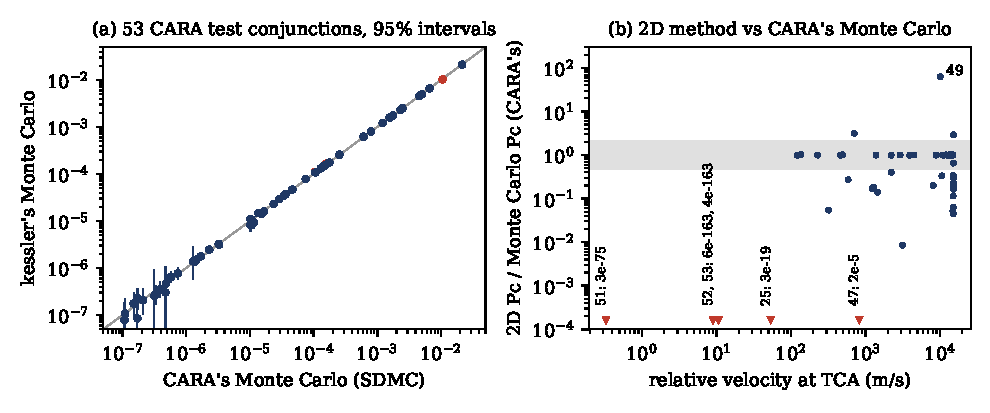
\includegraphics[width=\linewidth]{fig_agreement.pdf}
\caption{(a) Our Monte Carlo against CARA's on the 53 test conjunctions, with 95\% intervals on
both axes; red points have $|z|\ge2$. (b) CARA's own 2D probability divided by its own Monte
Carlo, against relative velocity at TCA; the grey band is a factor of two. Five cases fall
below the axis and are marked with their ratios.}
\label{fig:agreement}
\end{figure}

For each conjunction we ran enough trials for about 3,000 hits, or as many as fitted in 120~s on
4 CPU cores: \nTotalTrials{} billion trials in \nTotalMinutes{} minutes in all, against the
\nNasaTrials{} billion CARA ran. Figure~\ref{fig:agreement}a and Table~\ref{tab:summary} show
the result. The largest $|z|$ is \nMaxAbsZ; \nBeyondTwo{} cases have $|z|\ge2$, against 2.4 expected
by chance in 53, and the sum of squares is what agreement predicts. Our implementation of the 2D method itself matches CARA's 2D values to a relative
difference of at most \nMaxRelTwoD.

\begin{table}[t]
\centering\small
\caption{Agreement with CARA's two-body Monte Carlo (SDMC) on its 53 test conjunctions.}
\label{tab:summary}
\begin{tabular}{lr}
\toprule
Conjunctions with $|z|<2$ / $|z|<3$ & \nWithinTwo{} / \nWithinThree \\
Largest $|z|$ & \nMaxAbsZ \\
$\chi^2$ over all 53 (53 degrees of freedom) & \nChiSq{} ($p=\nChiP$) \\
Hits per case, ours: minimum / median & \nMinHits{} / \nMedianHits \\
Cases with fewer than 100 hits (ours) & \nFewHits \\
\bottomrule
\end{tabular}
\end{table}

\begin{table}[t]
\centering\small
\caption{Selected conjunctions: the 2D method, CARA's Monte Carlo and ours.}
\label{tab:cases}
\begin{tabular}{rlrrrrr}
\toprule
Case & Objects & $v_{\rm rel}$ & 2D (CARA) & CARA SDMC & This work & $z$ \\
\midrule
1 & Hubble, Delta 2 rocket body & 2.9 km/s & $6.11\times10^{-4}$ & $6.11\times10^{-4}$ & $6.23\times10^{-4}$ & $+0.9$ \\
25 & WorldView-2, Fengyun-1C debris & 53.6 m/s & $4.5\times10^{-23}$ & $1.51\times10^{-4}$ & $1.53\times10^{-4}$ & $+0.5$ \\
45 & ICESat-2, SpaceBEE-114 & 15.2 km/s & $3.3\times10^{-8}$ & $7.38\times10^{-7}$ & $7.7\times10^{-7}$ & $+0.3$ \\
49 & & 10.1 km/s & $2.4\times10^{-5}$ & $3.89\times10^{-7}$ & $3.6\times10^{-7}$ & $-0.5$ \\
51 & & 0.3 m/s & $4.5\times10^{-81}$ & $1.30\times10^{-6}$ & $1.4\times10^{-6}$ & $+0.2$ \\
52 & TROPICS Pathfinder, LINCS2 & 9.0 m/s & $6.5\times10^{-168}$ & $1.17\times10^{-5}$ & $9.3\times10^{-6}$ & $-1.6$ \\
53 & & 10.7 m/s & $3.9\times10^{-168}$ & $1.02\times10^{-5}$ & $8.3\times10^{-6}$ & $-1.4$ \\
\bottomrule
\end{tabular}
\end{table}

Table~\ref{tab:cases} shows the cases that make the test set hard. The 2D method underestimates
case 25 by a factor of $3\times10^{18}$ and the two drifting cases 52 and 53 by more than
$10^{160}$: at 9--11~m/s the objects stay close for a large fraction of an orbit, nothing about
the encounter is short or straight, and the 2D integral sees only a vanishing tail. It also
overestimates: case 49 by a factor of 63. Figure~\ref{fig:agreement}b shows the pattern over
all 53. The failures are not confined to slow encounters: of the 27 conjunctions above 10~km/s,
14 are off by more than a factor of two, up to 22 times too low and 63 times too high. The
Monte Carlo agrees with CARA's on these as on the others.

The test has limited power where hits are few. For the conjunctions with $\text{Pc} \sim
10^{-7}$, 120~s bought only tens of millions of trials, and \nFewHits{} cases have fewer than
100 hits (as few as \nMinHits). On those the comparison detects only gross disagreement; the
conjunctions that discriminate between modelling choices are run with far more trials in the
next section.

\section{Two choices that decide agreement}\label{sec:choices}

\paragraph{Sampling coordinates.} A linear covariance describes a Gaussian in some coordinates,
and its image in other coordinates is not Gaussian; the difference grows with the size of the
along-track uncertainty \cite{junkins1996}. Table~\ref{tab:sampling} draws the same three
conjunctions in three ways: Cartesian states, equinoctial elements with the semi-major axis
$a$, and equinoctial elements with the mean motion $n$. On case 1, a fast encounter with small
uncertainty, all three agree with CARA. On case 25 Cartesian sampling is 15\% low ($z=-3.7$):
a straight-line draw in position and velocity tilts each sample's velocity off its orbit, and
at 54~m/s that changes how long the objects stay close. On case 45, whose probability of
$7.4\times10^{-7}$ is decided by the far tail, Cartesian sampling finds no hit at all in
$10^8$ trials, where CARA's value predicts about 74. Equinoctial sampling, in either form,
reproduces that tail: with $10^9$ trials each, the semi-major-axis form gives \nTailPcA{}
($z=\nTailZA$) and the mean-motion form \nTailPcN{} ($z=\nTailZN$), against CARA's
$7.38\times10^{-7}$, and the two are indistinguishable at this precision (about $\pm4\%$). At
$10^8$ trials the mean-motion form had read 33\% high ($z=+2.8$, 98 hits), and an earlier,
smaller run had suggested the semi-major-axis form was high; neither survived ten times the
trials. With around a hundred hits, an excursion of two to three standard errors somewhere in a
table of comparisons is to be expected, and a claim about the far tail needs hits in the
hundreds.

\begin{table}[t]
\centering\small
\caption{Sampling coordinates, at the default window ($\pm P/2$, encounter at TCA only).
$z$ is against CARA's hits and trials.}
\label{tab:sampling}
\begin{tabular}{rlrrrr}
\toprule
Case & Gaussian in & Pc, this work & Hits / trials & CARA SDMC & $z$ \\
\midrule
\csname @@input\endcsname tab_sampling.tex 
\bottomrule
\end{tabular}
\end{table}

\paragraph{Window length and which encounter.} CARA's standalone \texttt{Pc\_SDMC} wrapper
defaults to a window of a quarter of the shorter period either side of TCA \cite{caratools}.
That is ample for fast encounters and too short for drifting ones (Table~\ref{tab:window}): on
cases 52 and 53, at 9 and 11~m/s, $\pm P/4$ finds no hit in $8\times10^6$ trials where CARA's
values predict about 90, because the objects approach so slowly that the hits happen more than a
quarter period from TCA. At $\pm P/2$ both agree with CARA's. At $\pm P$ both come out 40--50\%
higher ($z\approx+4.4$), and counting only the approach containing TCA does not change that: at
these speeds the times at which the two objects can come within reach form one unbroken span, so
there is no separate second encounter to exclude. For a drifting pair, the probability of
collision ``in this conjunction'' is not defined independently of the window, and the window
must be reported with the number. CARA's published values for these two cases correspond to
$\pm P/2$ in our implementation; we do not know the span CARA used to produce them. Where the
times of possible approach do separate, in \nSecondWindows{} of the 53 conjunctions within
$\pm P/2$, our implementation counts only the interval containing TCA.

\begin{table}[t]
\centering\small
\caption{Window length and which close approach is counted, on the two drifting conjunctions.}
\label{tab:window}
\begin{tabular}{rllrrrr}
\toprule
Case & Window & Counted & Pc, this work & Hits & CARA SDMC & $z$ \\
\midrule
\csname @@input\endcsname tab_window.tex 
\bottomrule
\end{tabular}
\end{table}

\section{Speed}\label{sec:speed}

CARA distributes its two-body Monte Carlo as a compiled library (\texttt{libsdmc\_linux.so},
built with Intel Fortran) with a C++ entry point \cite{caratools}. We built a driver around the
published library and ran it and our implementation on the same machine with the same states,
covariances, HBR and window ($\pm P/4$, the library's default), one core each and $10^6$ trials
per case (\texttt{bench/m3\_vs\_nasa\_lib.py}). Both give the same probabilities within
statistical error (largest $|z|$ \nLibMaxAbsZ).

\begin{table}[t]
\centering\small
\caption{Time for $10^6$ trials on one core, CARA's library and this work, same inputs.}
\label{tab:speed}
\begin{tabular}{rrrrr}
\toprule
Case & $v_{\rm rel}$ (m/s) & CARA library (s) & This work (s) & Ratio \\
\midrule
\csname @@input\endcsname tab_speed.tex 
\bottomrule
\end{tabular}
\end{table}

On encounters from 123~m/s to 14.5~km/s our implementation takes 1.6--1.9~s per million
trials where the library takes 29--31~s (Table~\ref{tab:speed}). Most of the difference comes
from the search windows of Section~\ref{sec:method}: a fast encounter can hit only in a few
seconds around TCA, and a trial needs to be propagated only there. On the slowest case run, 25 at
54~m/s, the window that can hit spans most of the revolution, and the advantage falls to
1.8\x. We did not study the library's internals, and the comparison measures the two programs
as distributed, on one machine.

\section{Limitations}

The method is two-body, as CARA's SDMC is; it does not model drag, solar pressure or
manoeuvres between the CDM epoch and the encounter, nor the cross-correlation corrections
CARA can apply. The Gaussian is a modelling assumption in whichever coordinates it is placed,
and the agreement shown here is agreement with CARA's choices, not with ground truth, which no
one has for these conjunctions. The 60~s step of the minimum-distance search assumes no two
separate minima of the range within one step. The search-window bound is first-order with a
margin; it changed no hit on synthetic encounters or on \nWcCases{} of CARA's conjunctions, but it
is not proven. The speed comparison
is one machine and seven conjunctions. For drifting encounters the probability depends on the
time window, and agreement on cases 52 and 53 is agreement at $\pm P/2$.

\section{Reproducing the results}

{\sloppy\noindent\texttt{make \&\& python bench/m3\_sdmc.py} reproduces Section~\ref{sec:results};
\texttt{python bench/m3\_ablations.py} and \texttt{bench/m3\_tail.py} Section~\ref{sec:choices};
\texttt{python bench/m3\_windows\_check.py} the search-window check;
\texttt{bench/m3\_vs\_nasa\_lib.py} Section~\ref{sec:speed} (with a checkout
of CARA Analysis Tools and Intel's Fortran runtime); \texttt{python paper/figures.py} regenerates
every number, table and figure in this paper from the results files. The CDMs are fetched from
CARA's repository at a pinned commit and are not redistributed.\par}

\paragraph{Acknowledgements.} I thank NASA CARA for publishing its test conjunctions, results
and library, without which this check would not be possible.

\bibliographystyle{plainnat}
\bibliography{refs}

\end{document}
